\documentclass[10pt]{beamer}
\usepackage{appendixnumberbeamer}
\usepackage{booktabs}
\usepackage[scale=2]{ccicons}
\usepackage{pgfplots}
\usepackage{xspace}
\usepackage{xcolor}
\usepackage{caption}

\usetheme[progressbar=frametitle]{metropolis}
\usepgfplotslibrary{dateplot}
\newcommand{\themename}{\textbf{\textsc{metropolis}}\xspace}
\captionsetup[figure]{labelformat=empty}

% ---------------------------------------------------------
\title{Artificial astrocyte networks}
% \subtitle{A modern beamer theme}
% \date{\today}
\date{}
\author{Erik J Peterson}
\institute{CoAxLab\\Carnegie Mellon University}

% ---------------------------------------------------------
\begin{document}
\maketitle

\begin{frame}{Table of contents.}
  \setbeamertemplate{section in toc}[sections numbered]
  \tableofcontents%[hideallsubsections]
\end{frame}

% ---------------------------------------------------------
\section[]{Goal.}
\begin{frame}[fragile]{Goal}
\begin{itemize}
    \item Use models and proof methods from artificial intelligence to try and set an \alert{upper bound} on astrocyte computation.
\end{itemize}
\end{frame}

% ---------------------------------------------------------
\section[ANNs]{What are artificial neural networks?}
\begin{frame}[fragile]{What are ANNs?}
\begin{itemize}
\item By example, using vision.
\item Sparse networks.
\end{itemize}
\end{frame}

\begin{frame}[fragile]{Visual digit recognition.}
\begin{columns}
\column{0.5\textwidth}
\centering
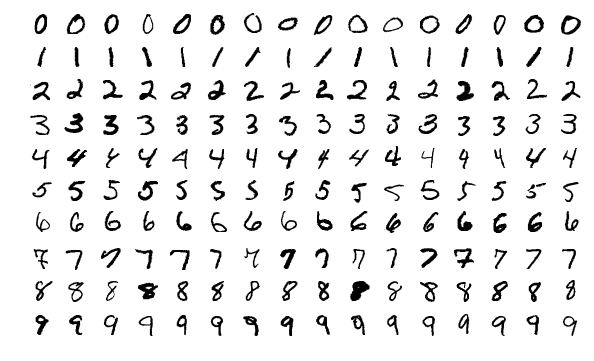
\includegraphics[scale=0.25]{images/minst.png}
\column{0.5\textwidth}
\centering
 = 1,2,3,4,5,6,\ldots
\end{columns}
\end{frame}

\begin{frame}[fragile]{What are ANNs?}
\begin{columns}
\column{0.5\textwidth}
\begin{figure}
    \centering
    
\includegraphics[scale=0.5]{images/nine_only.png} 
\end{figure}
\column{0.5\textwidth}
\centering
 $= 9$?
\end{columns}
\end{frame}


\begin{frame}[fragile]{What are ANNs?}
\begin{columns}
\column{0.5\textwidth}
\centering
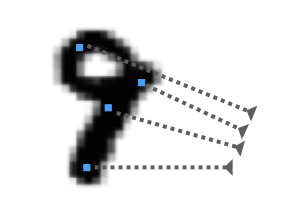
\includegraphics[scale=0.5]{images/nine_x.png} 
\column{0.5\textwidth}
\centering
 $\alert{\sum} x_{ij} = 9$
\end{columns}
\end{frame}

\begin{frame}[fragile]{What are ANNs?}
\begin{columns}
\column{0.5\textwidth}
\centering
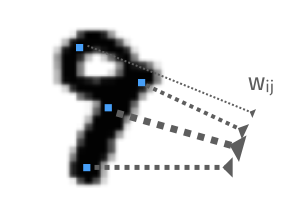
\includegraphics[scale=0.5]{images/nine_wx.png} 
\column{0.5\textwidth}
\centering
 $\sum \alert{w_{ij}} x_{ij} = 9$
\end{columns}
\end{frame}

\begin{frame}[fragile]{What are ANNs?}
\begin{columns}
\column{0.5\textwidth}
\centering
% 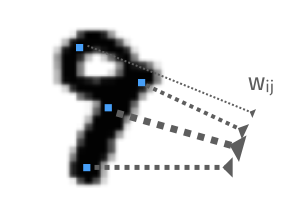
\includegraphics[scale=0.5]{images/nine_wx.png} 
\column{0.5\textwidth}
\centering
 $\sum w_{ij} x_{ij} + \alert{b_i} = 9$
\end{columns}
\end{frame}

\begin{frame}[fragile]{What are ANNs?}
\begin{columns}
\column{0.5\textwidth}
\centering
% 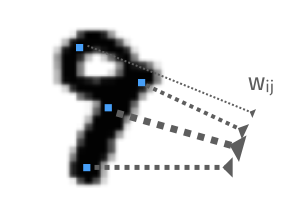
\includegraphics[scale=0.5]{images/nine_wx.png} 
\column{0.5\textwidth}
\centering
 $\alert{\phi}(\sum w_{ij} x_{ij} + b_i) = 9$
\end{columns}
\end{frame}

\begin{frame}[fragile]{What are ANNs?}
\begin{figure}
    \centering
    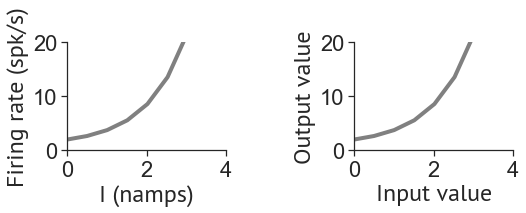
\includegraphics[scale=0.4]{images/phi.png}
    \caption{\textit{FI}-curve (left) $\approx$ $\alert{\phi}$ nonlinearity (right)}
\end{figure}
\end{frame}

\begin{frame}[fragile]{What are ANNs?}
\begin{figure}
    \centering
    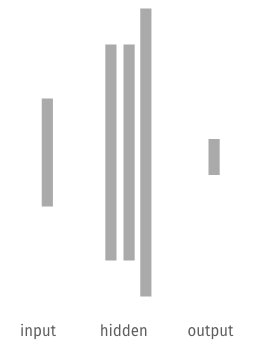
\includegraphics[scale=0.4]{images/deep.png}
    \caption{
    \alert{A deep ANN network}. Each box is a \textit{layer}: $\phi (\sum w_{ij} x_{ij} + b_i)$
    }
\end{figure}
\end{frame}

% ---------------------------------------------------------
\section[AANs]{Defining artificial astrocyte networks.}

\begin{frame}[fragile]{Basic astrocyte limits.}
\begin{itemize}
    \item No synapses
    \item No axons 
\end{itemize}
\end{frame}

\begin{frame}[fragile]{Basic astrocyte limits.}
\begin{itemize}
    \item No $w_i$
    \item No $\sum$
\end{itemize}
\end{frame}

\begin{frame}[fragile]{Basic astrocyte properties}
\begin{itemize}
    \item $[Ca^{2+}]$ dynamics
    \item Gliotransmission
\end{itemize}
\end{frame}

\begin{frame}[fragile]{Assumption 1 ($\phi$).}
\begin{figure}
    \centering
    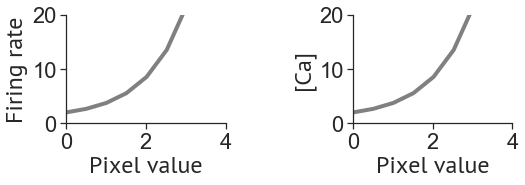
\includegraphics[scale=0.4]{images/phi_ca.png}
    \caption{Firing rate (left) $\leftrightarrow$ $[Ca^{2+}]$ dynamics (right)}
\end{figure}
\begin{itemize}
    \item 
\end{itemize}
\end{frame}

\begin{frame}[fragile]{Assumption 2 ($w_i$).}
\begin{columns}
\column{0.5\textwidth}
\begin{itemize}
    \item \alert{Directional} $[Ca^{2+}]$-dependent gliotransmission.
\end{itemize}
\column{0.5\textwidth}
    \centering
    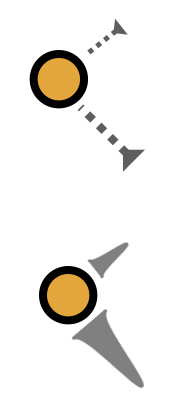
\includegraphics[scale=0.4]{images/gliotrans.jpeg}
\end{columns}
\end{frame}

\begin{frame}[fragile]{Assumption 3 ($\sum$).}
\begin{itemize}
    \item \alert{Directional} $[Ca^{2+}]$ waves, driven by gliotransmission.
\end{itemize}
\end{frame}

% ---------------------------------------------------------
\section[In theory.]{Theory.}
\begin{frame}[fragile]{Computational calcium waves.}
\begin{itemize}
\item Let's treat neurons only as a source of input; glia do all the computation!
\item Let's study a forward moving $[Ca^{2+}]$ wave.
\item With Assumptions 1-3\ldots
\item \alert{Prove}: it is a universal function approximator.
\end{itemize}
\end{frame}

\begin{frame}[fragile]{A universal function approximator?}
$|F(x) - f(x)| < \epsilon$
\end{frame}

\begin{frame}[fragile]{A universal function approximator?}
$|\alert{F}(x) - f(x)| < \epsilon$
\begin{itemize}
    \item[$\alert{F}(x)$] : any target function (whose domain is bounded)
\end{itemize}
\end{frame}

\begin{frame}[fragile]{A universal function approximator?}
$|\alert{F}(x) - f(x)| < \epsilon$
\begin{itemize}
    \item[$\alert{F}(x)$] : visual recognition system in cat (target)
\end{itemize}
\end{frame}

\begin{frame}[fragile]{A universal function approximator?}
$|F(x) - \alert{f}(x)| < \epsilon$ 
\begin{itemize}
\item[$F(x)$] : visual recognition system in cat (\textit{target})\\
\item[$\alert{f}(x)$] : an ANN (\textit{approximator})
% \item[] : $\phi (\sum w_{ij} x_{ij} + b_i)$
\end{itemize}
\end{frame}

\begin{frame}[fragile]{A universal function approximator?}
$|F(x) - f(x)| < \alert{\epsilon}$ 
\begin{itemize}
\item[$F(x)$] : visual recognition system in cat (\textit{target})\\
\item[$f(x)$] : an ANN (\textit{approximator})
% \item[] : $\phi (\sum w_{ij} x_{ij} + b_i)$
\item[$\alert{\epsilon}$] : the max error boundary
\end{itemize}
\end{frame}

\begin{frame}[fragile]{A universal function approximator?}
$|\alert{F}(x) - \alert{f}(x)| < \alert{\epsilon}$ 
\begin{itemize}
\item[] It is possible the target $\alert{F}$ and learned function $\alert{f}$ can be made arbitrarily close to $\alert{\epsilon}$.
\end{itemize}
\end{frame}


\begin{frame}[fragile]{Proof sketch.}
\begin{columns}
\column{0.5\textwidth}
\centering
\begin{figure}
    \centering
    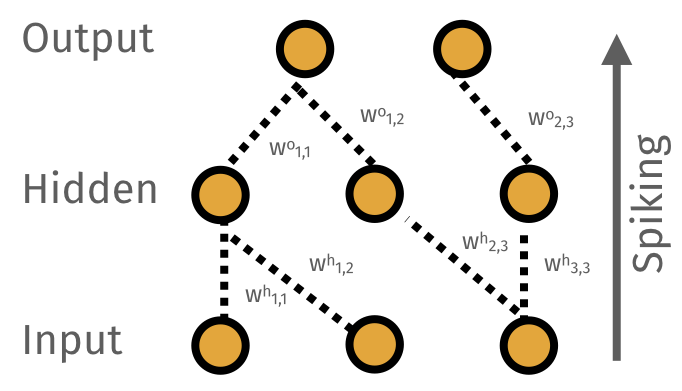
\includegraphics[scale=0.2]{images/ann.png}
    \caption{
    \begin{itemize}
        \item Bölcskei \textit{et al} (2019) $F$ can be approximated by $f$ in $M << N$ connections.
        \item $f$ : $\phi (\sum w_{ij} x_{ij} + b_i)$
    \end{itemize}}
\end{figure}
\column{0.5\textwidth}
\end{columns}
\end{frame}

\begin{frame}[fragile]{Proof sketch.}
\begin{columns}
\column{0.5\textwidth}
\centering
\begin{figure}
    \centering
    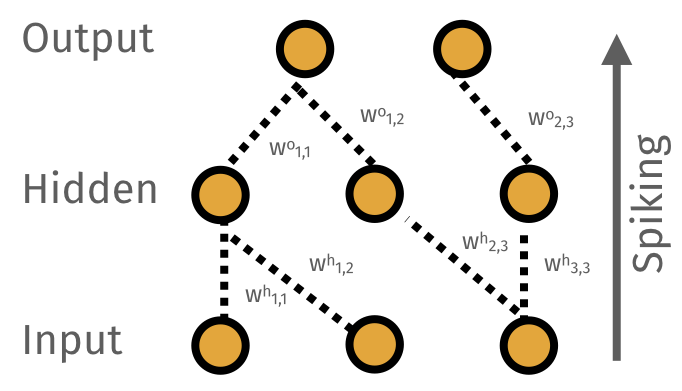
\includegraphics[scale=0.2]{images/ann.png}
    \caption{
    \begin{itemize}
        \item Bölcskei \textit{et al} (2019) $F$ can be approximated by $f$ in $M << N$ connections.
        \item $f$ : $\phi (\sum^M w_{ij} x_{ij} + b_i)$
    \end{itemize}}
\end{figure}
\column{0.5\textwidth}
\centering
\begin{figure}
    \centering
    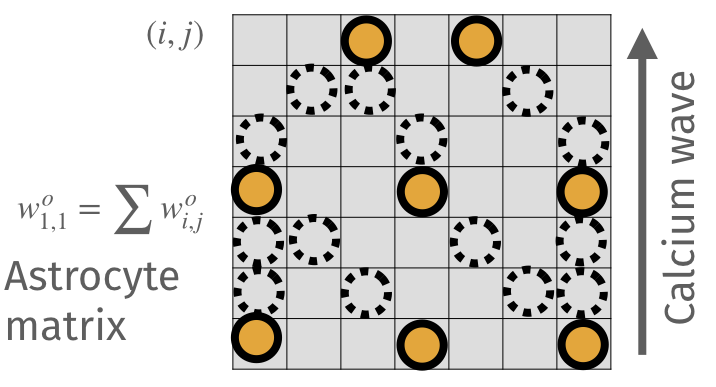
\includegraphics[scale=0.2]{images/aan.png} 
    \caption{
    \begin{itemize}
        \item Approximation of the universal approximator
        \item $w^o_{1,1} = \sum w_{i,j}^o$
        \item \alert{Astrocyte Sudoku}
    \end{itemize}}
\end{figure}
\end{columns}
\end{frame}

% ---------------------------------------------------------
\section[In practice.]{Practice.}
\begin{frame}[fragile]{Three astrocyte layers.}
\begin{columns}
\column{0.5\textwidth}
\begin{enumerate}
    \item Gather
    \item Slide
    \item Spread
\end{enumerate}
\column{0.5\textwidth}
\centering
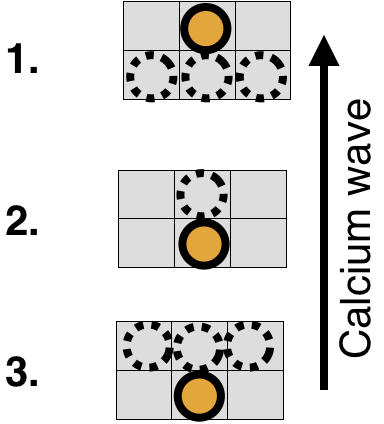
\includegraphics[scale=0.25]{images/layers.png} 
\end{columns}
\end{frame}

\begin{frame}[fragile]{An astrocyte network.}
\begin{figure}
    \centering
    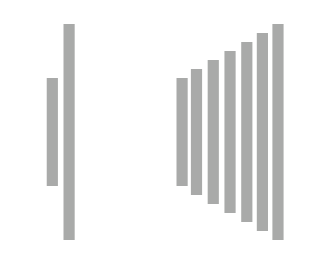
\includegraphics[scale=0.35]{images/glaidim.png} 
    \caption{
    \begin{itemize}
        \item Two equivilant neural (\textit{left}) and astrocyte networks (\textit{right}).
        \item For astrocyte computation \alert{width requires depth}.
    \end{itemize}}
\end{figure}
\end{frame}

\begin{frame}[fragile]{Methods.}
\begin{itemize}
    \item \alert{Task}: MINST digits
    \item \alert{Use}: \{\textit{slide}, \textit{spread}, \textit{gather}\} in pytorch
    \begin{enumerate}
        \item VAE, $N=(784,20)$
        \item Perceptron, $N=(20,30,10)$    
    \end{enumerate}
    \item Loss: Cross-entropy
    \item Optimizer: ADAM
\end{itemize}
\end{frame}

\begin{frame}[fragile]{Results.}
\begin{columns}
\column{0.4\textwidth}
    \centering
    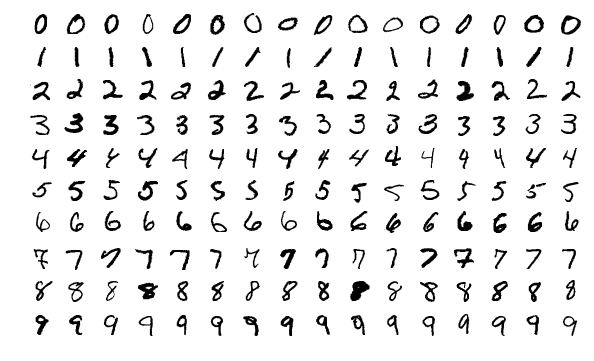
\includegraphics[scale=0.2]{images/minst.png} 
\column{0.6\textwidth}
\begin{figure}
    \centering
    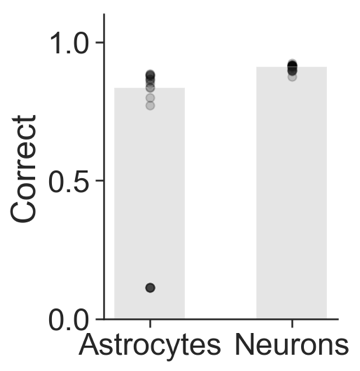
\includegraphics[scale=0.3]{images/results.png} 
    \caption{Test set performance (N=20 epochs)}
\end{figure}
\end{columns}
\end{frame}

% ---------------------------------------------------------
\section[Conclusions.]{Conclusions.}
\begin{frame}[fragile]{Conclusions.}
\begin{itemize}
\item AANs $\rightarrow$ universal function approximator.
\item AANs can solve hard vision problems.
\item An \alert{upper bound} for the performance of real astrocytes? 
\end{itemize}
\end{frame}

\begin{frame}[fragile]{Future work.}
\begin{itemize}
\item Upper bound $\rightarrow$ biological upper bound (\alert{help})
\item Recurrent waves (in collaboration)
\item Better motivated tasks (\alert{help})
\end{itemize}
\end{frame}

\begin{frame}[fragile]{Open science.}
\begin{itemize}
\item[Code] \url{github.com/CoAxLab/glia_playing_atari}
\item[Talk] \url{github.com/parenthetical-e/glia-talk-sfn-2019}
\item[] 
\item[] \alert{Thank you!}
\end{itemize}
\end{frame}


% ---------------------------------------------------------
% \begin{frame}[allowframebreaks]{References}
%   \bibliography{demo}
%   \bibliographystyle{abbrv}
% \end{frame}

% ---------------------------------------------------------
\end{document}
